\documentclass{article}

\usepackage[T1]{fontenc}
\usepackage[utf8]{inputenc}
\usepackage{graphicx}
\usepackage{caption}
\usepackage[font=small,labelfont=bf]{caption}
\usepackage{booktabs, siunitx}
\usepackage{tikz}
\usepackage{tikz-qtree}
\usepackage{pifont}
\usepackage[margin=0.90in]{geometry}
\usepackage{etoolbox,titling}
\usepackage{enumitem}
\usepackage{fancyhdr}
\usepackage{soulutf8}
\usepackage{epigraph}
\usepackage{amssymb}
\usepackage{amsmath}

\pagestyle{fancy}
\fancyhf{}
\rhead{Chiara Solito}
\lhead{Dispense di Laboratorio di Bioinformatica}
\rfoot{Pagina \thepage}
\lfoot{Bioinformatica - A.A. 2021/22}
\usetikzlibrary{trees}
\tikzstyle{every node}=[draw=black,thick,anchor=west]
\newcommand{\angstrom}{\mbox{\normalfont\AA}}

\begin{document}
\newcommand\tab[1][0.3cm]{\hspace*{#1}}


\begin{titlepage}
    \begin{center}
        \vspace*{1cm}
            
        \Huge
        \textbf{Vaccine Supervision}
            
        \vspace{0.5cm}
        \LARGE
        Progetto di Ingegneria del Software
            
        \vspace{1.5cm}
            
        \textbf{Virginia Filippi e Chiara Solito}

        \vspace{0.8cm}

            
        \Large
        Corso di Laurea in Bioinformatica\\
        Università degli studi di Verona\\
        A.A. 2021/22
            
    \end{center}
\end{titlepage}
La presente è la documentazione blablabla.\\
Insieme a questo documento in formato PDF viene fornito anche il codice \LaTeX  con cui è stato generato.
\tableofcontents
\thispagestyle{empty}
\newpage
\thispagestyle{empty}

\section{Traccia dell'Elaborato}
\section{Analisi e Specifica dei Requisiti}
(\dots )\\
\subsection{Specifiche casi d'uso}
In questa sezione definiamo le proprietà dell'applicazione.\\
Come dichiarato nella traccia il sistema prevede l'utilizzo da parte di due tipologie di personale medico: Medico e Farmacologo. 
Entrambi i tipi di utente possono utilizzare l'applicazione dopo opportuno login: in questa sede si è previsto che gli utenti siano pre-registrati da un amministratore di sistema esterno (sul modello di sistemi medici già noti). Non è stato quindi previsto un form di registrazione, durante lo sviluppo.
\begin{figure}[htp]
    \centering
    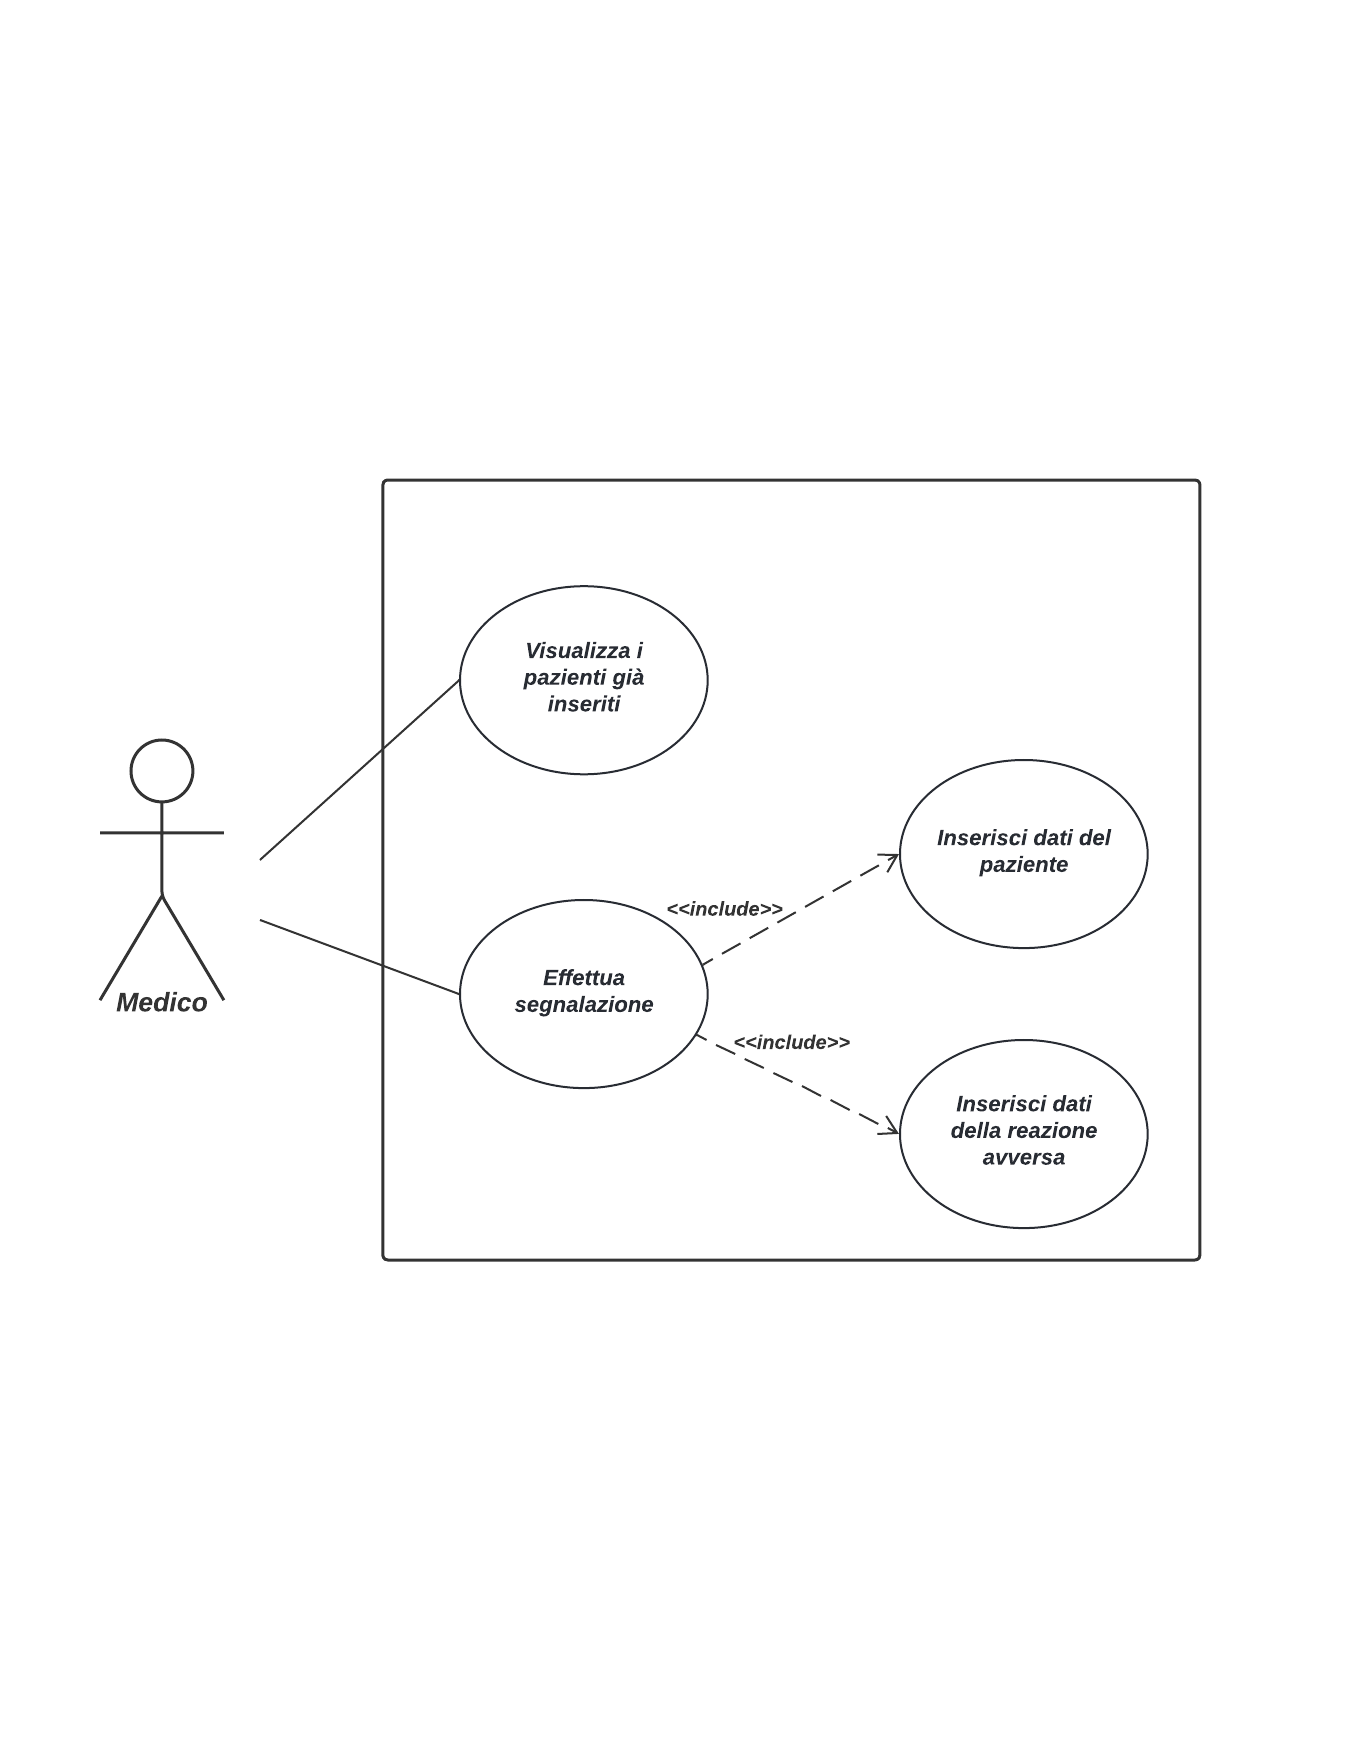
\includegraphics[width=0.7\textwidth]{pictures/CasoDUsoMedico_SfondoTrasparente.png}
    \caption{Caso d'uso Medico}
\end{figure}

\end{document}